%! suppress = MissingImport
\chapter{Introduction}
\label{cha:introduction}

%\todo[inline]{Electric vehicles are the future}
On today's day and age, the global concern on climate
change has been a major focus on recent international agreements,
such as the Paris Agreement \citep{parisAgreement},
incentivizing many car manufacturers to introduce
\gls{EVs} as the eco-friendly
solution for sustainable transport for the future.

As \gls{EVs} have been growing in popularity in
recent years, car manufacturers have
increased competitiveness on vehicle's performance
\citep{evCompetitiveness}, a decisive factor 
for consumers \citep{EGBUE2012717}.

A vehicle's autonomy also known as \gls{eRange},
allows consumers to know an estimate on the
remaining driving distance for the existing \gls{EV}
battery power, easing driver's anxiety for the duration
of a trip to a charging station.

The \gls{eRange} can be estimated through many
driving data parameters,
such as vehicle design, driver's behavior, whether,
road inclination and \gls{SOC} estimation.
The \gls{eRange} accuracy allows consumers to rely
on its vehicle for longer travel time and efficient
charging plans, \gls{eRange} estimation
however, is a complex problem which has prompted
previous studies in the past to provide a solution 
\citep{classicEVX, predictionOfeRange}.

\vbox {
    \todo[inline]{relate with "Prediction of electric
    vehicle range: A comprehensive review of current issues and challenges"}
    Prior work \citep{classicEVX} on \gls{eRange}
    estimation demonstrated that using a
    history-based algorithm on am adaptive model
    provides a more reliable \gls{eRange} prediction
    than a basic \gls{SOC} - manufacturer data relation,
    this is mainly due to taking into account the
    vehicle's driving history.
}

%\todo[inline]{TODO: Mensionar IA na atualidade}
Machine learning is often a viable tool for complex
problems, this is due to its nature of 
learning from previous data to 
gradually achieve better results.
As its broad use on a large variaty of problems 
is vast and could be applied to most problems
\citep{mitchelllearning}, the \gls{eRange}
 estimation problem could be one of which, 
through the use of \gls{machineLearning}, 
achieve better results \cite{predictionOfeRange},
requiring an initial phase to learn from 
the model and then estimate through real-time \gls{SOC} variations.
This project approaches the \gls{eRange} estimation
problem with the use of \gls{machineLearning} based
model to increase its accuracy.

%\todo[inline]{What will be done}
The proposed solution is divided into three phases: 
a \gls{dataset} generation phase, a learning phase
and an estimation phase.
On the \gls{dataset} generation phase, a \gls{dataset}
will be created from historical traffic dataset
from personally recorded vehicle trips as well as
external existing datasets such as \textit{VED} \citep{vedDataset}
 \todo{remove VED dataset if not valid}
as well was an external library that generates 
\gls{EV} trip and consumption \gls{timeSeries} \citep{emobpy}.
The resulting dataset contains multiple
trips with their respective vehicle power consumption [kW]
and the vehicle speed [km/h] in a  \gls{timeSeries} format.
This \gls{dataset} will be used to train the model
on the learning phase through machine learning, 
allowing it to learn the estimation of 
the \gls{eRange} for each trip on the \gls{dataset}.
After training the model with the dataset,
the estimation phase performs the \gls{eRange} prediction
on live \gls{SOC} monitoring of a driving \gls{EV}.
The following figures represent an overview of the system:

%! suppress = MissingLabel
% \begin{figure}[H]
%     \begin{center}
%         %! suppress = MissingLabel
%         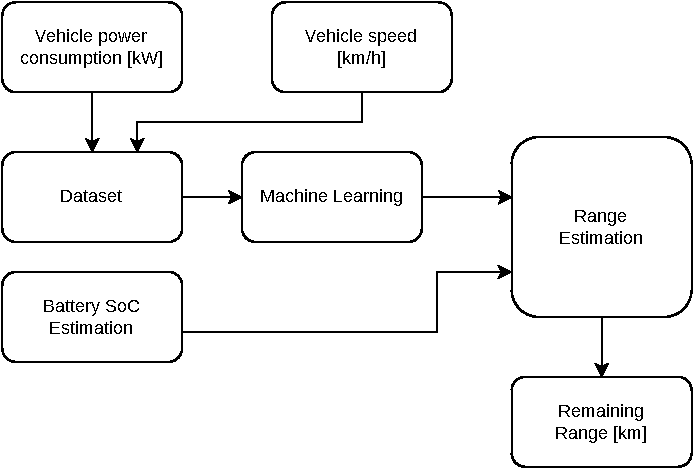
\includegraphics[scale=1.0]{../figures/generic_diagram}
%         \caption{System overview.}
%     \end{center}
% \end{figure}

\begin{figure}[H]
    \begin{center}
        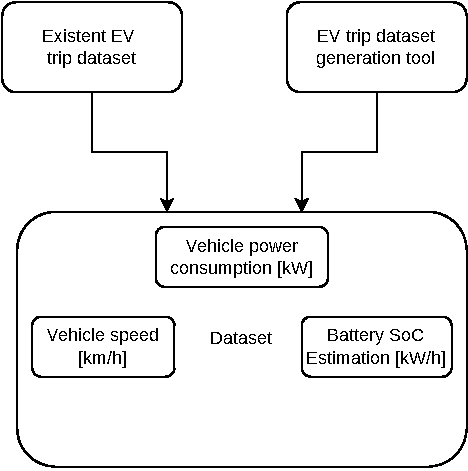
\includegraphics[scale=1.0]{../figures/generic_diagram_dataset_generation_phase}
        \caption{System overview - Dataset generation.}
    \end{center}
\end{figure}

\begin{figure}[H]
    \begin{center}
        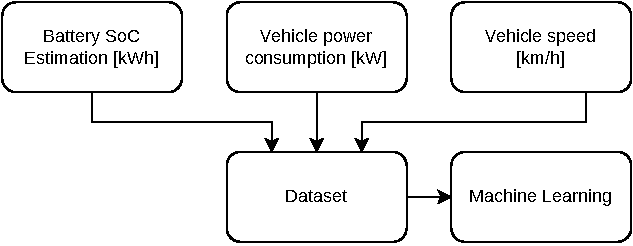
\includegraphics[scale=1.0]{../figures/generic_diagram_learn_phase}
        \caption{System overview - Learning phase.}
    \end{center}
\end{figure}

\begin{figure}[H]
    \begin{center}
        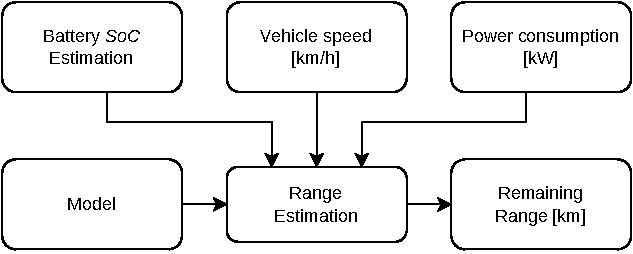
\includegraphics[scale=1.0]{../figures/generic_diagram_estimation_phase}
        \caption{System overview - Estimation phase.}
    \end{center}
\end{figure}
